In this section we introduce a coin flip functionality \Fflip and discuss how composition affects its import requirements, and we introduce a design pattern where session types can enforce message ordering across multiple channels. 
\Fflip is realized by protocol $\prot{flip}$ in the $\F_{\msf{comauth}}$-hybrid world (a functionality combining \Fcom with a one-way, one-shot channel, \Fauth, from the receiver to the sender). 
In this section we again go through assigning consatnt import but this time notice how import assignments change when, say, a functionality is used by different protocols. 
%We push the realizing protocols, simulators, and process code to Appendix~\ref{app:flip} and focus here on the \Fflip and \Fropp session types.

\begin{figure*}
	\begin{center}
	\parbox{0cm}{
	\begin{tabbing}
		$\m{flip[K]\{n\}\{m\}} = \ichoice{\mb{init}: \rpaypot{n} \; K \arrow \ichoice{\mb{getflip}: \rpaypot{n}  \echoice{ $\=$\mb{yes}: \rgetpot{m} \; Bit \product 1,$ 
		$ \mb{no}: \rgetpot{m} \; \m{flipped}[K]}}}$ \\
		$\m{receiver[K]\{n\}\{m\}} = \ichoice{\mb{getflip}: \rpaypot{n} \; \echoice{$\=$ \mb{yes}: \rgetpot{m} \; Bit \product 1,$
		$\mb{no}: \rpaypot{m} \; \m{receiver[K]}}}$ \\
		$\m{adv[K]\{n\}} = \echoice{\mb{askflip}: \; K \arrow \echoice{\mb{flipok}: \ichoice{$\=$\mb{yes}: 1,$
		$\mb{no}: 1}}}$
	\end{tabbing}}
	\end{center}
	\vspace{-5mm}
	\caption{The session types describing \Fflip's channels with the flipper, receiver, and the adversary.}
	\label{fig:fliptype}
\end{figure*}

The code for \Fflip is quite simple and shown below and the types \inline{flipper} and \inline{receiver} shown in Figure~\ref{fig:fliptype}.
\begin{lstlisting}[basicstyle=\scriptsize\BeraMonottFamily, frame=single, mathescape]
$\nproc$ F_coinflip[K]{p2fn}{m} :
  (k: Int), (rng: [Bit]), (sid: session[1]),
  ($\$$F: flipper[$\tp{K}$]{$\tp{p2fn}$}{$\tp{f2pn}$}), ($\$$R: receiver[$\tp{K}$]{$\tp{p2fn}$}{$\tp{f2pn}$}),
  ($\$$A: adv[$\tp{K}$]) |- ($\$$c: 1) =
{
  $\ncase$ $\$$F (
    init =>
      x = $\nrecv$ $\$$F ;
      $\nget$ $\$$F {p2fn}
      b = sample 1 rng ;
      $\$$A.flipped ;
      $\nsend$ $\$$A x ;
      $\tg{(* wait for getflips *)}$
      $\$$f <- getflip_f{$\tp{p2fn}$}{$\tp{f2pn}$} <- b $\$$F ;
      $\$$r <- getflip_r[$\tp{K}$]{$\tp{p2fn}$}{$\tp{f2pn}$} <- b x $\$$R ;
  )
}

$\nproc$ getflip_f[K]{p2fn}{m} :
  (k: Int), (rng: [Bit]), (sid: session[s]),
  (b: Bit), ($\$$F: f_flipped[$\tp{K}$]{$\tp{p2fn}$}{$\tp{f2pn}$}),
  ($\$$A: adv[$\tp{K}$]) |- ($\$$c: 1) =
{
  $\ncase$ $\$$F (
    getflip =>
      $\$$A.askflip ;
      $\ncase$ $\$$A (
        yes => 
          $\$$F.yes ; $\nsend$ $\$$F b ;
          $\npay$ {f2pn} K $\$$F ;
        no => $\$$F.no ; $\npay$ {f2pn} K $\$$F ;
      )
  )
}
\end{lstlisting}
The code for  \inline{getflip_r} is identical except it is the receiver. 
It checks for a flip result by either party, \Fflip asks the adversary whether to deliver the output to the party asking for it.
Much like the real-world case where if the corrupt committer never opens its commitment, the simulator here can ensure that only the flipper receives the flip.
As the session type indicates, the adversary responds with a \inline{yes} or \inline{no} to deliver the flip.

\subsection{Protocol for Flipping}
The protocol we use to realize the coin flip uses \Fcom, used throughout this work, and a one-way channel $\F_{\msf{auth}}$ which allows messages to be sent in both directions. 
Its type differs from \Fcom alone.
Again we split communication between two uni-direction channels for each of the committer and receiver unlike \Fcom.
The types of the channels are
\begin{center}
\parbox{0cm}{
\begin{tabbing}
	$\m{commitp2f}[a]\{m\} = $\\
	\qquad $\ichoice{$\=$\mb{commit}: \rpaypot{2} Bit \product \m{committedp2f}[a]}$ \\
    	%\>$\mb{sendmsg}: \rpaypot{m} a \product \m{commitp2f}[a]}$ \\
	$\m{committedp2f}[a]\{m\} = $\\
	\qquad $\ichoice{$\=$\mb{open}: \m{donep2f}[a]}$ \\
		%\>$\mb{sendmsg}: \rpaypot{m} a \product \m{committedp2f}[a]}$ \\
	$\m{commitf2p}[a] = \echoice{\mb{msg}: \rgetpot{m} a \arrow \m{commitf2p}[a]}$ \\
	$\m{receivep2f}[a] = \ichoice{\mb{sendmsg}: \rpaypot{m} a \product \m{receivep2f}[a]}$ \\
	$\m{receivef2p}[a] = \echoice{$\=$\mb{committed}: \m{receivedf2p}[a]}$\\
		%\>$\mb{msg}: \rgetpot{m} a \arrow \m{receiverf2p}[a]}$ \\
	$\m{receivedf2p}[a] = \echoice{$\=$\mb{opened}: Bit \arrow \m{donef2p}[a]}$ \\
	    %\>$\mb{msg}: \rgetpot{m} a \arrow \m{receivedf2p}[a]}$ \\
\end{tabbing}}
\end{center}
Again, this type is seen by wrapped instances of \prot{flip} and, as far as the commitment inputs, is the same type that \Fcom sees (we use different names here to distinguish channels). 

%Notice that the ordering of messages locally for the committer and receiver are still present. 
Notice that the inputs for the committer have not changed, and it additionally has a channel to receive messages from the channel functionality. 
Like the example of $\pi_\msf{com}$ above, we can set the parameters as necessary for $\prot{flip}$.
As you'd expect the commitment functionality takes in some amount of non-zero import, here it's 2 for the random oracle assumption we're working with, to ensure that it's able to perform some polynomial amount of work in computing hashes, 
and that the \mb{sendmsg} branches take an arbitrary amount of import allowing a sender to send $m$ import to the other party. 

The protocol that realizes this functionality, $\pi_{\msf{commauth}}$ is identical to $\pi_{\msf{com}}$ except it forwards $\mb{sendmsg}$ messages to the hybrid functionality \Fropp' that allows for \emph{2-way} communication, that is one-shot in each direction, rather than the original one-way channel. 
Notice that \Fropp' has a two-way channel, because $\pi_{\msf{commauth}}$ will send messages from committer to receiver and vice versa, but the high level $\F_{\msf{commauth}}$ only exposes the new feature of sending messages from the receiver to the committer. 
Getting to the two-way channel from \Fropp only requires the following on top of the session type in Figure~\ref{fig:fropptype}: 
\begin{itemize}
	\item an additional $\mb{sendmsg}$ on \m{rquery} that allows sending 1 import to the committer
	\item and \mb{msg} session in \m{shash} with 1 import token to let the committe receive messages.
\end{itemize}

Again we aim to set the constant amount of import that is sent through \partywrapper with \Z and \F. 
Like the original commitment, the \partywrapper, running wrapped instances of \prot{flip}, needs sends 4 units of import to $\F_{\msf{commauth}}$ on \mb{commit}, \mb{open}, and \mb{sendmsg} inputs due to the protocl that we are using. 
Additionally, the one-way message carrying the randomness $r$ from the receiver to the comitter which, by virtue of the 4 import for the commitment, must result in the \partywrapper sending 4 import to $\F_{\msf{commchan}}$.

Given these import requirements, we can assign a sufficient assignment of import that the \partywrapper receives from \Z. 
We conclude that a constant of 12 import per input from \Z is sufficient to accomdate all $\F_{\msf{commchan}}$ inputs including the message sent from the receiver. 

We elide similar reasoning and assignment for communication betwen the \partywrapper and \A because it is much simpler, however it is clear to see that it is easy to determine such assignments and conclude that the providerless channels construction, import-wise, does not conflict with the generalized composition operator.
All the import assigned here, both for the sessio types seen by the wrapped protocol parties and the constant amounts sent to/from the \partywrapper, are checked and validated by the NomosUC type system. 

%\subsection{Simulator}
%The protocol for the coin flip uses \Fcom. 
%The flipper commits to a bit $b$, the receiver sends the flipper a random bit $r$ in return, the flipper opens its commitment, and both parties compute the flip as $r \oplus b$.
%The simulator for this protocol to realize \Fflip is straightforward:
%\begin{itemize}
%\item If the flipper is corrupt, the simulator tells the flipper to \inline{init} the flip when the environment sends it a \inline{Commit b} message. It gets the flip outcome $f$ from the flipper and simulates the receivers random bit $r = f \oplus b$ for the environment. It never delivers the flip outcome to the receiver unless the environment instructs it to open the flipper's commitment. By setting $r = f \oplus b$, when the environment receives $f$ it can check that $r \oplus b = f$.
%\item If the receiver is corrupt, the simulator waits for \Fflip to inform it that the flip was initiated. It simulates the \inline{Commit} message from \Fcom to the receiver, for \Z. When it receives the random bit that \Z wants the receiver to send, it gets the flip outcome from the receiver, computes $b = r \oplus f$ and sends \inline{Open b} to \Z. Again, \Z can verify $b \oplus r$ similar to the above case.
%nl
%\end{itemize}
%
%\subsection{Composition}
%We describe a composition theorem in the previous section, a composition operator for protocols, and a brief highlight of the composition operator for simulators.
%Composition of the coin flip with the commitment protocol is realized with simulator composition in exactly this way.
%We give a diagram of simulator composition in~\ref{fig:simcomp}.
%\begin{figure}
%\centering
%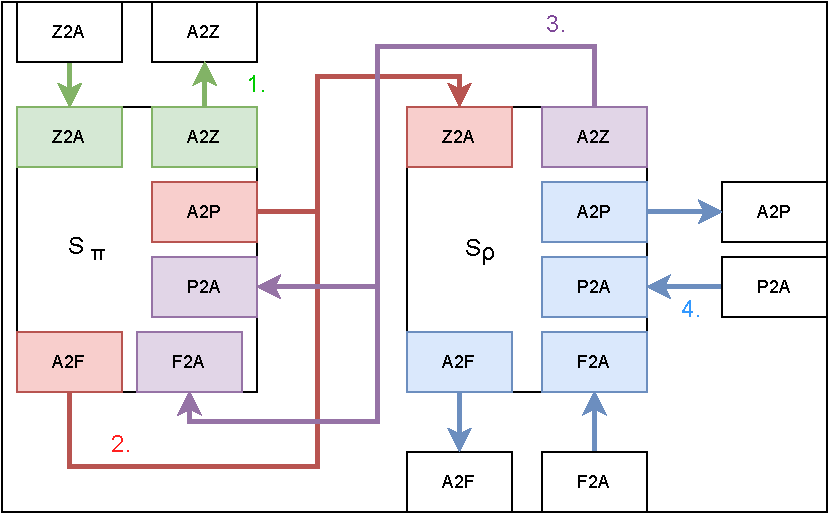
\includegraphics[scale=0.5]{figures/simcomp.pdf}
%\caption{The composed simulators for $\F_1 \xrightarrow{\rho \circ \pi} \F_3$. The real world consists of $(\rho \circ \pi, \F_1)$. Inputs from \Z are for $\F_1$ and dummy parties interacting with $\F_1$, which \SIM{\pi} is equipped to handle. Outputs from \SIM{\pi} are for $\F_2$ and dummy parties of $\F_2$ which \SIM{\rho} is equipped to handle. Finally, outputs from \SIM{\rho} are for $\F_3$ and dummy parties of $\F_3$, which is just the ideal world in Theorem~\ref{thm:composition}.}
%\label{fig:simcomp}
%\end{figure}
